%%%%%%%%%%%%%%%%%%%%%%%%%%%%%%%%%%%%%%%%%
% Beamer Presentation
% LaTeX Template
% Version 1.0 (10/11/12)
%
% This template has been downloaded from:
% http://www.LaTeXTemplates.com
%
% License:
% CC BY-NC-SA 3.0 (http://creativecommons.org/licenses/by-nc-sa/3.0/)
%
%%%%%%%%%%%%%%%%%%%%%%%%%%%%%%%%%%%%%%%%%

%----------------------------------------------------------------------------------------
%	PACKAGES AND THEMES
%----------------------------------------------------------------------------------------

\documentclass{beamer}

\mode<presentation> {

% The Beamer class comes with a number of default slide themes
% which change the colors and layouts of slides. Below this is a list
% of all the themes, uncomment each in turn to see what they look like.

%\usetheme{default}
%\usetheme{AnnArbor}
%\usetheme{Antibes}
%\usetheme{Bergen}
%\usetheme{Berkeley}
%\usetheme{Berlin}
%\usetheme{Boadilla}
%\usetheme{CambridgeUS}
%\usetheme{Copenhagen}
%\usetheme{Darmstadt}
%\usetheme{Dresden}
%\usetheme{Frankfurt}
%\usetheme{Goettingen}
%\usetheme{Hannover}
%\usetheme{Ilmenau}
%\usetheme{JuanLesPins}
%\usetheme{Luebeck}
%\usetheme{Madrid}
%\usetheme{Malmoe}
%\usetheme{Marburg}
%\usetheme{Montpellier}
%\usetheme{PaloAlto}
%\usetheme{Pittsburgh}
%\usetheme{Rochester}
%\usetheme{Singapore}
%\usetheme{Szeged}
\usetheme{Warsaw}

%\usecolortheme{albatross}
%\usecolortheme{beaver}
%\usecolortheme{beetle}
%\usecolortheme{crane}
%\usecolortheme{dolphin}
%\usecolortheme{dove}
%\usecolortheme{fly}
%\usecolortheme{lily}
%\usecolortheme{orchid}
%\usecolortheme{rose}
%\usecolortheme{seagull}
\usecolortheme{seahorse}
%\usecolortheme{whale}
%\usecolortheme{wolverine}

\usefonttheme{professionalfonts} 
\setbeamertemplate{caption}[numbered]
%\usetheme{}

\addtobeamertemplate{navigation symbols}{}{%
    \usebeamerfont{footline}%
    \usebeamercolor[fg]{footline}%
    \hspace{1em}%
    \insertframenumber/\inserttotalframenumber
}

\usepackage[utf8]{inputenc}
\usepackage[english]{babel}
\usepackage{physics}
\usepackage{amsmath}
\usepackage{bm}
\usepackage{amsfonts}
\usepackage{amssymb}
\usepackage{caption}
\usepackage{subcaption}
\usepackage{float}


%\setbeamertemplate{footline} % To remove the footer line in all slides uncomment this line
%\setbeamertemplate{footline}[page number] % To replace the footer line in all slides with a simple slide count uncomment this line

%\setbeamertemplate{navigation symbols}{} % To remove the navigation symbols from the bottom of all slides uncomment this line
}

\usepackage{graphicx} % Allows including images
\usepackage{booktabs} % Allows the use of \toprule, \midrule and \bottomrule in tables

%----------------------------------------------------------------------------------------
%	TITLE PAGE
%----------------------------------------------------------------------------------------

\title[13. Chaotic Magnetic Pendulum]{Problem no.13 - Chaotic Magnetic Pendulum}
\subtitle{IPT 2022}
\author[University of Ljubljana]{Team Slovenia \\ Presenter: Rok Grgič Meško}
\date{\vspace{-5ex}}

\begin{document}

\begin{frame}

\begin{figure}[H]
	\centering
	  
\includegraphics[width=\textwidth]{naslovnica_ipt.png}
\end{figure}

\titlepage % Print the title page as the first slide

\vspace{-13mm}
\begin{figure}[H]
	\flushleft
	  
\includegraphics[width=6cm]{fmf_logo.png}
\end{figure}

\end{frame}


%----------------------------------------------------------------------------------------
%	PRESENTATION SLIDES
%----------------------------------------------------------------------------------------

%------------------------------------------------


\begin{frame}

\begin{block}{Official Problem Statement}
Consider a pendulum consisting of a magnetic bob attached to a string. If the pendulum is allowed to swing over a structure of permanent magnets, it will display complex motion. Study the pendulum dynamics and its dependence on the number of permanent magnets and their arrangement.
\end{block}

\end{frame}

%------------------------------------------------

\begin{frame}

\begin{block}{Hypotheses}
For certain initial parameters pendulum will display chaotic motion.
\end{block}

\end{frame}

%------------------------------------------------

\begin{frame}

\frametitle{Theory}
\begin{itemize}
\item
For continuous dynamical systems, the Poincaré–Bendixson theorem shows that chaos only exist in 3 dimensions described by non-linear equations.
\item
Dynamical chaos can exist in systems starting with effective 3/2 (1/2 for no explicit time dependence) degrees of freedom.
\item
Integrals of motion (conserved) restrict the solution and make dynamical chaos less likely:
\[ N_F = \dfrac{1}{2} (N - N_{int}) \]
\end{itemize}

\end{frame}

%------------------------------------------------

\begin{frame}

\frametitle{Theory}

\begin{itemize}
\item Chaotic pendulum:
\[ N = 4, \quad N_{int} = 1 \Rightarrow N_F = 3/2 \]
\end{itemize}

In the presence of dissipation, a mechanical system relaxes down to one of its local energy minima.
Generally, dissipation tends to make chaotic motion regular.

\end{frame}

%------------------------------------------------

\begin{frame}

\frametitle{Theoretical Description}
We approximate magnets by magnetic dipoles.\\
Coordinate system origin at the top of the string.\\
Force between two dipoles:
\begin{gather}
%
\begin{split}
\mathbf{F_m}(\mathbf{r'}, \mathbf{m}_1, \mathbf{m}_2) = \dfrac{3 \mu_0}{4 \pi r'^5} \Big [ (\mathbf{m}_1\cdot\mathbf{r'})\mathbf{m}_2 + (\mathbf{m}_2\cdot\mathbf{r'})\mathbf{m}_1 + \\
+ (\mathbf{m}_1\cdot\mathbf{m}_2)\mathbf{r'} - \dfrac{5(\mathbf{m}_1\cdot\mathbf{r'})(\mathbf{m}_2\cdot\mathbf{r'})}{r'^2}\mathbf{r'} \Big ]
\end{split}
\end{gather}
\begin{gather}
\textbf{r} = \left( x, y, - l - h + \sqrt{l^2 - x^2 - y^2} \right)
\end{gather}

All forces:
\begin{gather}
\mathbf{F} = \mathbf{F_g} + \mathbf{F_{mi}} - \mathbf{F_v}
\\
\mathbf{F} = \mathbf{F_g} + \mathbf{F_{mi}} - \langle \mathbf{F_g} + \mathbf{F_{mi}} \, , \dfrac{\mathbf{r}}{r} \rangle \dfrac{\mathbf{r}}{r}
\end{gather}

\end{frame}

%------------------------------------------------

\begin{frame}

\frametitle{Theoretical Description}

Dimensionless:
\begin{gather}
\{x, y, z\} = L \{\chi, \gamma, \zeta\}, \qquad \bm r = L \bm \rho, \qquad t = T \tau
\\
\lVert \mathbf{m_1} \rVert = \lVert \mathbf{m_2} \rVert
\\
L = \sqrt[4]{\dfrac{\mu_0 \lVert \mathbf{m_1} \rVert^2}{mg}}, \qquad T = \sqrt{\dfrac{L}{g}}
\\
\begin{split}
\mathbf{\mathcal{F}_{mi}}(\bm \rho, \bm \rho_i') = \dfrac{3}{4 \pi \rho_i'^5} \Bigg [ (-\dfrac{\bm \rho}{\rho}   \cdot \bm \rho_i')\mathbf{\hat{e}}_z + (\mathbf{\hat{e}_z} \cdot\bm \rho_i')-\dfrac{\bm \rho}{\rho} +  \\
 + (-\dfrac{\bm \rho}{\rho}\cdot\mathbf{\hat{e}}_z) \bm \rho_i' - \dfrac{5(-\dfrac{\bm \rho}{\rho}\cdot \bm \rho_i')(\mathbf{\hat{e}}_z\cdot \bm \rho_i')}{\rho_i'^2} \bm \rho_i' \Bigg]
\end{split}
\end{gather}

\end{frame}

%------------------------------------------------

\begin{frame}

\frametitle{Theoretical Description}

Dimensionless:
\begin{gather}
\bm \rho = \left( \chi, \gamma, - \lambda - \eta + \sqrt{\lambda^2 - \chi^2 - \gamma^2} \right)\\
\mathbf{\mathcal{F}} = \mathbf{\mathcal{F}_g} + \mathbf{\mathcal{F}_{mi}} - \mathbf{\mathcal{F}_v}
\\
\mathbf{\mathcal{F}} = \mathbf{\mathcal{F}_g} + \mathbf{\mathcal{F}_{mi}} - \langle \mathbf{\mathcal{F}_g} + \mathbf{\mathcal{F}_{mi}} \, , \dfrac{\bm \rho}{\rho} \rangle \dfrac{\bm \rho}{\rho}
\end{gather}

Projection on x, y plane.

\begin{gather}
 \mqty(\ddot{\chi} \\ \ddot{\gamma}) = \mqty(\langle \mathbf{\mathcal{F}}, \, \hat{e}_x \rangle \\ \langle \mathbf{\mathcal{F}}, \, \hat{e}_y \rangle)
\end{gather}

We solve for $\chi, \gamma$.


\end{frame}

%------------------------------------------------


\begin{frame}

\frametitle{Experiment}
\begin{itemize}
\item
We used different magnetic configurations.
\item
We filmed throws at different initial parameters.
\end{itemize}
\begin{figure}[H]
	\centering
	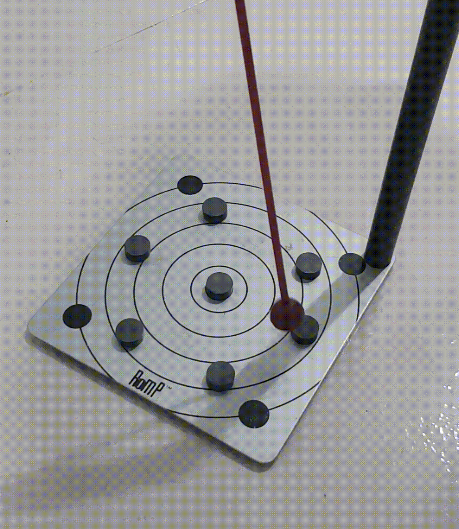
\includegraphics[width=0.3\textwidth]{srednja_kin_odbojna.png}
	  \caption{Example of an experiment.}
\end{figure}

Residual flux density on surface $B_r$
\begin{gather*}
m_1 = \dfrac{B_r V}{\mu_0} \approx 0.1 \mathrm{A m^2}, \quad l = 0.18 \mathrm{cm}, \quad h = 0.02 \mathrm{cm}, \quad m \approx 3 \mathrm{g}
\end{gather*}


\end{frame}

%------------------------------------------------

\begin{frame}

\frametitle{Experiment}
We found three regimes.

\begin{itemize}
\item High kinetic energy:\\
\qquad pendulum swings sinusoidally in a regular way.
\item Medium kinetic energy:\\
\qquad pendulum swings chaotically.
\item Low kinetic energy:\\
\qquad perturbed sinusoidal swinging in a minimum (spherical \\
\qquad pendulum).
\end{itemize}


\end{frame}

%------------------------------------------------

\begin{frame}

\frametitle{Results form simulation}
Experiment videos\\
Animation $\rightarrow$

\begin{figure}[H]
	\centering
	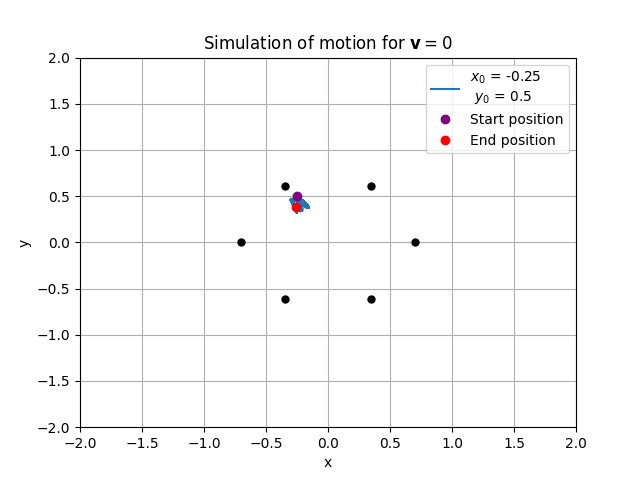
\includegraphics[width=0.7\textwidth]{motion 18.png}
	  \caption{Example of stationary point.}
\end{figure}

\end{frame}

%------------------------------------------------


\begin{frame}

\frametitle{Results form simulation}

\begin{figure}[H]
	\centering
	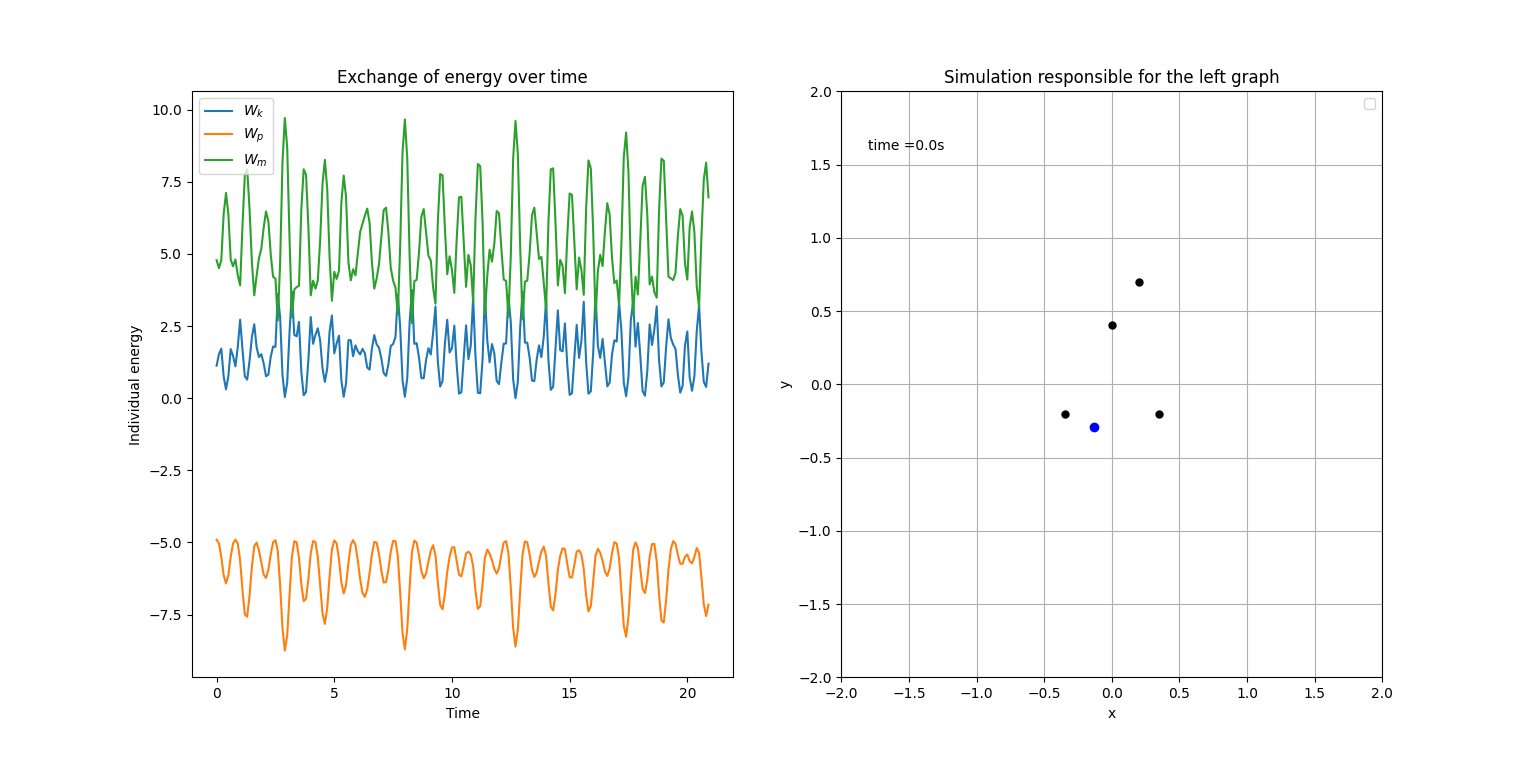
\includegraphics[width=1.2\textwidth]{energy.png}
	  \caption{Exchange of energy over time.}
\end{figure}

\end{frame}

%------------------------------------------------


\begin{frame}

\frametitle{Results form simulation}

\begin{figure}[H]
	\centering
	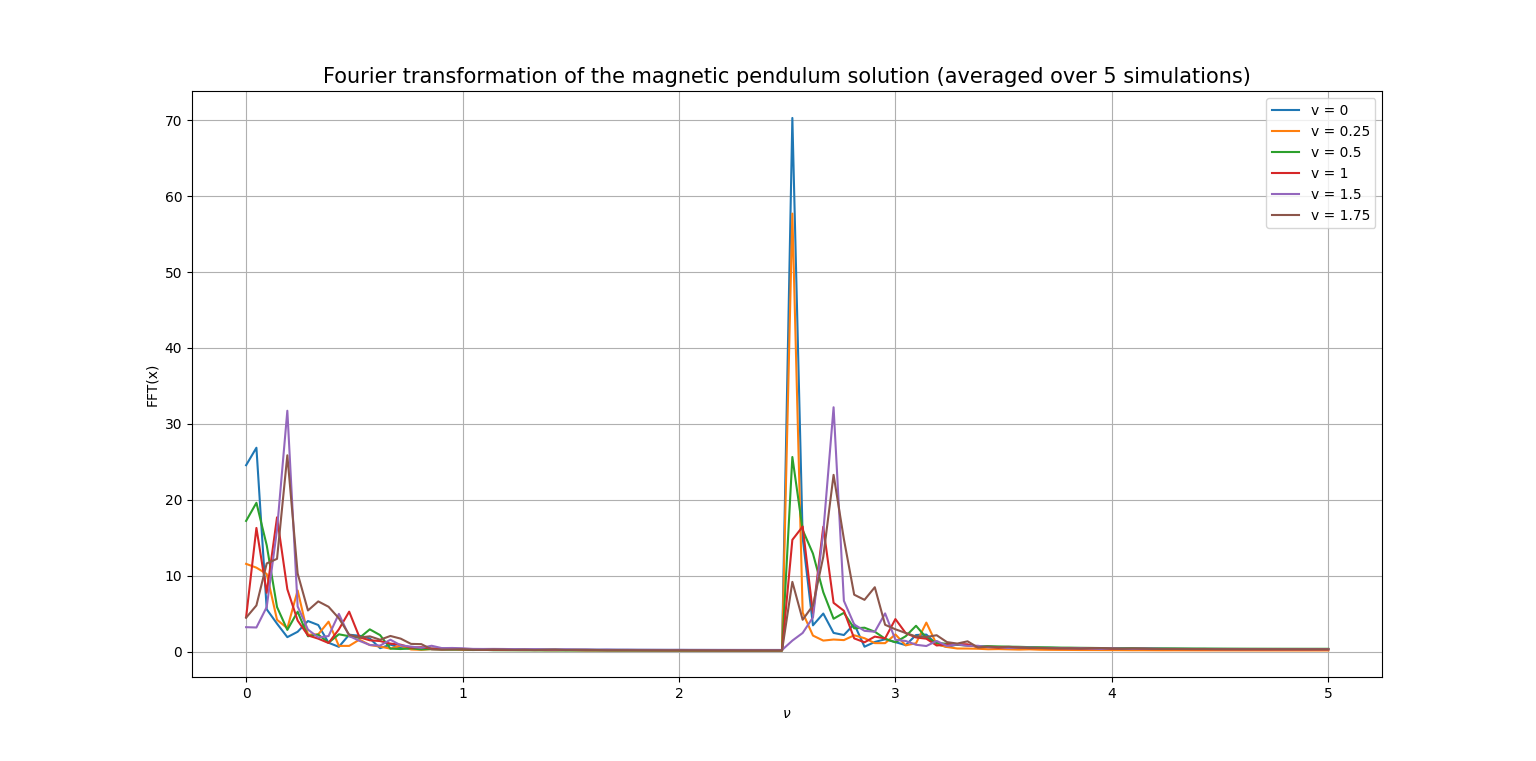
\includegraphics[width=1.1\textwidth]{fourier.png}
	  \caption{Fourier transformation, eigen frequencies. For higher energies motion is more chaotic. Second peak is redundant, arises form discrete model.}
\end{figure}

\end{frame}

%------------------------------------------------


\begin{frame}

\frametitle{Results form simulation}

\begin{figure}[H]
	\centering
	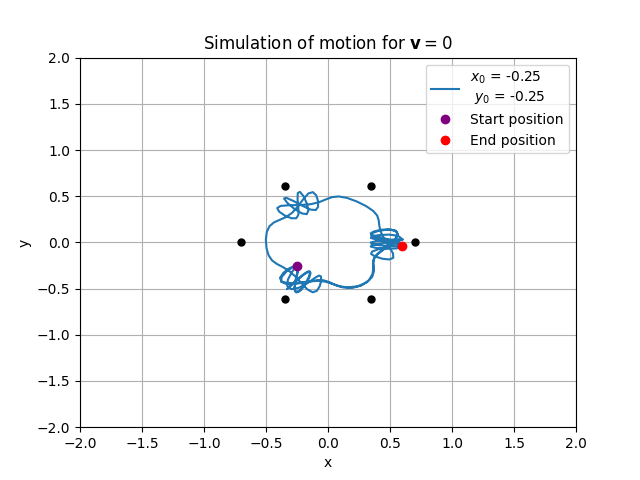
\includegraphics[width=0.8\textwidth]{motion 15.png}
	  \caption{Motion looks like a random walk. Swinging in a minimum and jumping to other minimums.}
\end{figure}

\end{frame}

%------------------------------------------------

\begin{frame}
\frametitle{Conclusion}

\begin{itemize}
\item We found regular and chaotic regimes of motion in experiment.
\item We showed in simulation that for certain initial parameters motion is chaotic.

\end{itemize}

\end{frame}

%------------------------------------------------

\begin{frame}

\frametitle{References}

\setbeamertemplate{bibliography item}[text]

\begin{thebibliography}{9}

\bibitem{clanek}
D. Garanin. \textit{Dynamical Chaos}. (2008). \url{https://www.lehman.edu/faculty/dgaranin/Mechanics/Dynamical_Chaos.pdf}


\end{thebibliography}

\end{frame}

%------------------------------------------------

\end{document} 